\section{Desktop Environment and Design Language}
\label{sec:desktop}

The desktop environment is the most visible part of the system and the primary
differentiator for users switching from other platforms. The goal is a fast,
coherent desktop that does not feel like a collection of independent projects
assembled by different teams in different decades. The stack reflects this:
performance-critical and system-close code is Rust, everything visual is
TypeScript with Tailwind CSS, and the two halves communicate over well-defined
interfaces that neither side reaches past.

\subsection{Architecture and IPC}
\label{sec:desktop-ipc}

Three communication channels connect the compositor core to the shell and its
frontend, each carrying a different class of data. Figure~\ref{fig:shell-ipc}
shows the structure.

\begin{figure}[htbp]
\centering
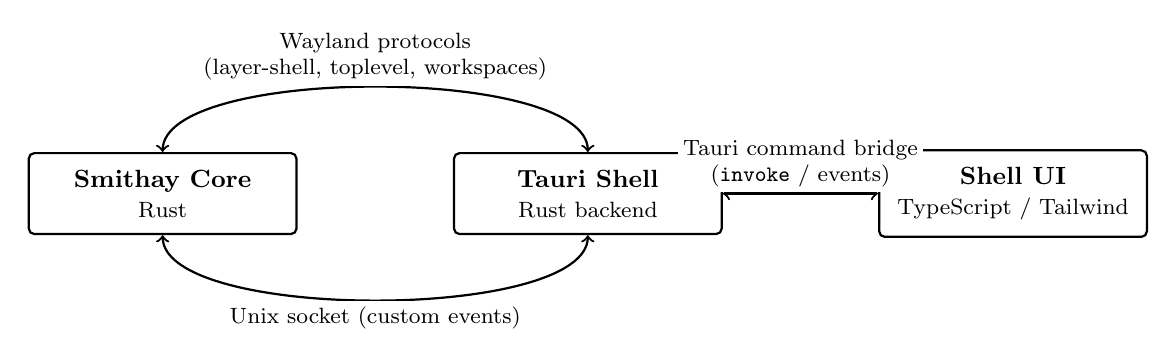
\begin{tikzpicture}[
  box/.style={
    draw, thick, rectangle, rounded corners=2pt,
    minimum width=3.4cm, minimum height=0.9cm,
    font=\small, align=center, inner sep=6pt
  },
  arr/.style={<->, thick},
  lbl/.style={font=\footnotesize, fill=white, inner sep=2pt, align=center},
]

\node[box] (smithay) at (0,   0) {\textbf{Smithay Core}\\{\footnotesize Rust}};
\node[box] (tauri)   at (5.4, 0) {\textbf{Tauri Shell}\\{\footnotesize Rust backend}};
\node[box] (ui)      at (10.8,0) {\textbf{Shell UI}\\{\footnotesize TypeScript / Tailwind}};

\draw[arr] (smithay.north) .. controls +(0,1.1) and +(0,1.1) .. 
  node[lbl, above] {Wayland protocols\\(layer-shell, toplevel, workspaces)} (tauri.north);

\draw[arr] (smithay.south) .. controls +(0,-1.1) and +(0,-1.1) ..
  node[lbl, below] {Unix socket (custom events)} (tauri.south);

\draw[arr] (tauri) -- node[lbl, above] {Tauri command bridge\\(\texttt{invoke} / events)} (ui);

\end{tikzpicture}
\caption{Shell IPC architecture. Wayland protocols carry window management data
(open windows, focus, workspace state). The Unix socket carries system-specific
events with no Wayland equivalent: theme updates, module lifecycle events,
graph notifications. The Tauri command bridge connects the Rust backend to the
TypeScript frontend within the shell process.}
\label{fig:shell-ipc}
\end{figure}

Wayland protocol extensions are the correct channel for anything the Wayland
ecosystem has standardized. The Unix socket exists for everything that does not
have a protocol equivalent and where a custom solution is both simpler and more
direct. Messages on the socket use JSON during development, with migration to
protobuf planned once the schema stabilizes.

Within the Tauri shell, the Rust backend and TypeScript frontend communicate
through Tauri's typed command system: the frontend calls Rust via
\texttt{invoke()}, Rust pushes events to the frontend via Tauri's event
emitter. No ad-hoc serialization; the bridge handles it.

\subsection{Compositor and Window Manager}
\label{sec:compositor}

The Wayland compositor is built on \emph{Smithay}, a Rust framework that
provides the low-level plumbing for compositor development: Wayland protocol
handling, DRM/KMS interfaces for direct display access, input processing via
libinput, and buffer management. Compositor logic such as window placement,
focus rules, and workspace behaviour is built on top of Smithay rather than
dictated by it. Building a compositor without a framework is an undertaking
that would dominate development for years; Smithay provides the foundation
without constraining the design. The COSMIC desktop compositor from System76
(cosmic-comp) is a useful reference for a Rust-first desktop project with
comparable goals.

Window management supports both floating and tiling layouts, switchable per
workspace. There is no forced paradigm: users who prefer floating windows on
one workspace and a tiling layout on another can configure that independently
per workspace.

The compositor implements the Wayland protocol extensions listed in
Table~\ref{tab:wayland-protocols}.

\begin{table}[htbp]
\caption{Implemented Wayland protocol extensions}
\label{tab:wayland-protocols}
\begin{tabularx}{\linewidth}{lX}
\toprule
\textbf{Protocol} & \textbf{Purpose} \\
\midrule
\texttt{wlr-layer-shell}                  & Positions the taskbar and panels at screen edges, above application windows \\
\texttt{wlr-foreign-toplevel-management}  & Exposes open windows (title, app ID, state) to the taskbar \\
\texttt{wlr-workspace-management}         & Workspace state and control for the taskbar \\
\texttt{xdg-shell}                        & Standard protocol for normal application windows \\
\texttt{xdg-output}                       & Monitor metadata for multi-monitor configurations \\
\texttt{xdg-desktop-portal}               & Screensharing, file picker, and OS-level dialogs for sandboxed apps \\
\bottomrule
\end{tabularx}
\end{table}

\paragraph{XWayland.}
X11 compatibility is provided via XWayland, an X11 server that runs as a
Wayland client, making legacy X11 applications transparent to the user. It
starts on demand when the first X11 application launches and shuts down when
none are running. Users who do not need X11 compatibility can disable it in
Settings to reduce the attack surface.

XWayland has structural limitations that cannot be solved at the compositor
level and are documented rather than hidden. Copy-paste between X11 and
Wayland applications requires a clipboard synchronization bridge. Drag and drop
across protocol boundaries is unreliable. X11 applications cannot use
\texttt{xdg-desktop-portal} for screensharing and see only the XWayland
surface. Most significantly, X11 has no inter-application isolation: one X11
application can read the input events of any other X11 application, which is a
keylogger-class capability. This is recorded in the audit log whenever X11
applications are active.

\subsection{Shell and Application Framework}
\label{sec:shell}

The shell, comprising the taskbar, app launcher, notification center, quick
settings panel, and lock screen, is built with Tauri using TypeScript and
Tailwind CSS for the interface layer. Tauri renders the UI in a WebKitGTK
WebView, which gives the shell access to the full set of modern web rendering
capabilities without the memory cost of an Electron-style approach. The shell
is a Wayland client that uses \texttt{wlr-layer-shell} to anchor its surfaces
to screen edges.

\paragraph{ui-kit.}
A shared TypeScript package provides the visual foundation for every
first-party application. It is based on \emph{shadcn/ui}, a set of
Tailwind-based components that are copied into the project and fully owned
rather than consumed as an npm dependency. The package is organized in three
layers: design tokens as CSS custom properties that define the visual language
and propagate everywhere when changed; base components such as Button, Input,
Dialog, and Card built on shadcn/ui and styled with those tokens; and
system-specific components such as \texttt{WindowChrome}, \texttt{AppShell},
and \texttt{NotificationToast} that implement OS-level interaction patterns.
Every first-party application imports from ui-kit and receives visual
consistency without duplicating any of this infrastructure.

\paragraph{os-sdk.}
A shared Rust crate provides system integration to every first-party
application. It bundles a Graph Daemon client, an Event Bus client, MCP server
boilerplate, and the TOML-based config system. A new first-party application
starts with Tauri, ui-kit, and os-sdk and has graph access, event emission,
an MCP server, config handling, and a consistent UI without writing any
infrastructure code. The standard application layout reflects this:

\begin{lstlisting}[language=bash, caption={Standard first-party app structure}]
app-files/
  src-tauri/
    Cargo.toml        # includes os-sdk
    src/
      main.rs         # Tauri setup
      commands.rs     # Tauri command handlers
      mcp.rs          # this app's MCP server
  src/
    main.tsx
    components/       # app-specific components (uses ui-kit)
    pages/
\end{lstlisting}

\subsection{Spotlight}
\label{sec:spotlight}

Spotlight is the system-wide launcher and command palette: the primary
keyboard-driven entry point to the entire desktop, triggered by the Super key
by default and accessible from any context as a centered overlay. It handles
app launching, file and web search, inline calculation, unit conversion,
timezone lookup, and contextual actions derived from the current selection or
active application. It is not a file manager; deep folder navigation and bulk
operations belong in the File Manager. Spotlight surfaces the result the user
wants immediately or hands off to the right application.

When the AI layer is active, Spotlight gains an AI mode toggled by Tab.
Natural language queries are interpreted by the AI layer, resolved against the
Knowledge Graph and available MCP actions, and returned as structured results
in the same interface. Asking "show me what I worked on this week" is a
Spotlight query, not a file search.

Third-party modules can register as \texttt{spotlight.provider} to add result
types or as \texttt{spotlight.action} to add commands, as described in
Chapter~\ref{sec:modules}.

\subsection{Multi-Monitor and HiDPI}
\label{sec:multimonitor}

Wayland treats multi-monitor and HiDPI as first-class concepts: each output
carries its own scale factor, every Wayland-native application queries its
output properties and renders at the correct scale automatically, and
WebKitGTK respects the Wayland scale factor transparently. This means Tailwind
layouts render identically on 4K and 1080p without extra work in the
application.

The taskbar runs as a separate \texttt{layer-shell} surface per monitor, each
correctly sized and scaled for its output. Monitor configuration, covering
resolution, refresh rate, scale factor, position, and rotation per display, is
stored in \texttt{\textasciitilde/.config/display/config.toml} and applied at
compositor startup. When a new monitor is connected, the compositor checks for
a saved configuration and applies it immediately if found; for an unknown
monitor it applies sensible defaults and surfaces a notification offering to
open the display settings.

Fractional scaling at 1.5x (common on 1440p displays) uses the
\texttt{wp-fractional-scale-v1} Wayland protocol. Applications that implement
the protocol render crisply at fractional scales; those that do not are
rendered at the nearest integer scale, which results in slightly soft output
but is acceptable and documented. XWayland has no per-monitor DPI concept and
uses a single global DPI matched to the primary monitor; X11 applications do
not re-scale when moved between monitors, which is a structural X11 limitation
with no compositor-level fix.

\subsection{Design Language and Theming}
\label{sec:theming}

The specific visual design language, exact color palettes, and motion design
are finalized in a separate design phase. This section documents the technical
theming architecture: how themes are structured, how they propagate, and how
community themes work.

\paragraph{Token system.}
All themes are defined in TOML and compiled to platform-specific outputs by
the build system. The TOML file is the single source of truth; no theme value
exists anywhere else. From one \texttt{tokens.toml}, the build generates CSS
custom properties for the Tauri shell and all first-party applications, a GTK4
CSS theme, a Wine \texttt{.msstyles} file for Windows compatibility, and base
dark/light palettes for GTK3 and Qt. Changing the accent color in the TOML
propagates to every layer on the next build.

\paragraph{Built-in themes.}
Four themes ship with the system. Dark and Light are standard high-contrast
variants. High Contrast targets WCAG AAA at a minimum 7:1 contrast ratio, with
no transparency effects, no gradients, and no information conveyed through
color alone; it is generated from the same token system as the others and has
both a dark and light variant. Panda is the default and the most distinctive:
a deliberate split-surface design where different UI regions are intentionally
dark or light based on their function, creating a high-contrast frame around
bright content. The exact palette values for all four themes are determined in
the design phase; the token structure that generates them is fixed.

\paragraph{GTK and Qt coverage.}
GTK4 receives a full custom theme generated from tokens, covering the standard
set of interactive components with recognizably the same design language as the
first-party applications, though not pixel-perfect parity. GTK3 and Qt receive
fixed base dark and light themes only; the split-surface Panda design requires
component-level CSS control that neither framework provides cleanly, so they
fall back to whichever base is closer to the active theme.

\paragraph{Store themes.}
Community themes are distributed through the Store. A theme package declares
which layers it covers in its manifest and can inherit from any built-in theme,
overriding only the values it changes. The Store displays coverage clearly
before installation so users know which layers remain at the base theme. Two
authoring formats are supported: token overrides for authors who want to change
colors and radius values without touching CSS, and full compiled CSS for themes
that need structural changes beyond what the token system exposes. Both formats
can coexist in one package.

\paragraph{Live switching.}
Figure~\ref{fig:theme-chain} shows the theme inheritance chain. When the user
applies a theme, the Settings daemon loads the package, merges its token
overrides with the base theme, broadcasts new CSS custom properties to all
running Tauri processes (which update instantly without a reload), regenerates
and applies the GTK4 theme if the package covers it, and updates Wine prefix
themes if applicable. Token-based switches complete in under a second;
GTK4 regeneration may take one to two seconds on slower hardware.

\begin{figure}[htbp]
\centering
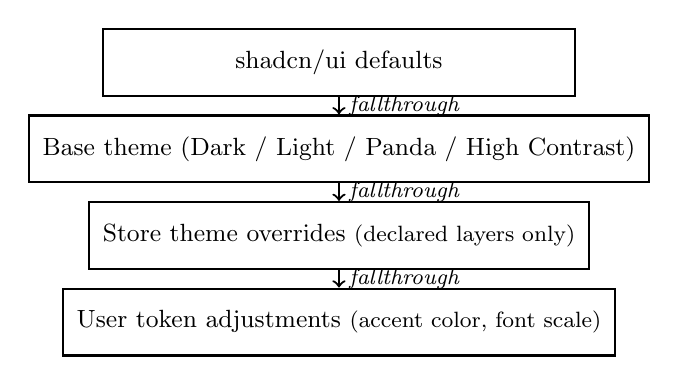
\begin{tikzpicture}[
  box/.style={
    draw, thick, rectangle,
    minimum width=6cm, minimum height=0.85cm,
    font=\small, align=center, inner sep=5pt
  },
  arr/.style={->, thick},
  lbl/.style={font=\footnotesize\itshape, anchor=west},
]

\def\sep{1.1}

\node[box] (shadcn) at (0, 3*\sep)
  {shadcn/ui defaults};
\node[box] (base)   at (0, 2*\sep)
  {Base theme (Dark / Light / Panda / High Contrast)};
\node[box] (store)  at (0, \sep)
  {Store theme overrides \footnotesize(declared layers only)};
\node[box] (user)   at (0, 0)
  {User token adjustments \footnotesize(accent color, font scale)};

\draw[arr] (shadcn) -- node[lbl, right] {fallthrough} (base);
\draw[arr] (base)   -- node[lbl, right] {fallthrough} (store);
\draw[arr] (store)  -- node[lbl, right] {fallthrough} (user);

\end{tikzpicture}
\caption{Theme inheritance chain. Each layer overrides only what it declares;
everything else falls through to the layer below. A Store theme that covers
only the shell and GTK4 leaves Wine and Qt at the base theme.}
\label{fig:theme-chain}
\end{figure}
